\documentclass[a4paper,12pt]{article}

\usepackage{graphicx}
\usepackage{subfig}
\usepackage{ucs}
\usepackage[utf8x]{inputenc}
\PrerenderUnicode{åäöÅÄÖ}

\title{Costanza Userguide}
\author{M. Green, P. Krupinski, P. Melke, P. Sahlin, H. Jonsson}

\begin{document}

\maketitle

%\abstract 

\section{Introduction}
This document describes how to use COnfocal STack ANalyZer Application
(Costanza), an ImageJ\cite{Abramoff2004} plugin for analyzing
stacks of image data. Such data come very often from confocal microscopy and that is where Costanza should prove to be most useful. The main purpose of Costanza is to segment nuclei marked cells
in three dimensions, making available quantitative measures such as
positions, sizes, and average intensities of GFP markers for the
segmented compartments. However since user is given the control on the parameters used by Costanza filters and image processors, they may be tweaked and combine freley to give good results also for other image processing task. The main algorithm is independent of intensity
thresholds, allowing for segmentation of data of varying intensity.

Costanza assumes a greyscale stack of images as input. It gives the user the possibility to use ImageJ x, y, and z scales for the stack or define custom ones. The results are thus displayed in real length units. 

\section{Installation instructions}
In order to use Costanza you must have ImageJ
(http://rsb.info.nih.gov/ij) installed on your system. Download the
file Costanza.zip from

http://www.thep.lu.se/\~{}henrik/Costanza/
Unzip the Costanza archive in the plugins directory of your ImageJ
installation. Next time you start ImageJ the plugin will show up as Costanza
in the Plugins drop down menu.

\section{Algorithms}
The algorithms provided in Costanza can be divided into the main
segmenting algorithm, preprocessing, and post-processing. Important feature of Costanza is the fact that all the algorithms operate in three dimensions instead of performing tasks on the set of two dimensional images. This increases the complexity and times of calculations but contributes to much more reliable results of segmentation and analysis, and is real strength of Costanza in comparison to other tools.

\subsection{Steepest gradient descent for segmentation}
This is the main algorithm for Costanza. It starts at each voxel in the stack
and tries to find local intensity maximum by ``walking'' uphill in intensity landscape
among its neighbors. All paths leading to the same maximum are saved to the
basin of attractor of this maximum, and represent a compartment. If more than one neighbor
has an intensity value higher then the current voxel, a step is performed to
the neighbor with highest

\begin{equation}
\frac{\Delta I}{\Delta \mathbf{x}} =
\frac{I_{neigh}-I_{current}}{\mathbf{x}_{neigh}-\mathbf{x}_{current}}
\end{equation}
where $\mathbf{x}_{current}(\mathbf{x}_{neigh})$ is the current (neighbor)
position, and $\mathbf{I}_{current}(\mathbf{I}_{neigh})$ are the respective intensities.
The neighborhood of the voxel can be chosen either as the six closest voxels, 	\textit{i.e.}
$(x\pm1,y,z)$, $(x,y\pm1,z)$, and $(x,y,z\pm1)$ or as all the twenty six surrounding voxels $\{(\{x,x\pm1\},\{y,y\pm1\},\{z,z\pm1\})\}-(x,y,z)$.

Optionally the treatment of intensity plateaus as one maximum can be turned on. This helps with analysis of data where large regions of identical intensities are present by choosing the maximum voxel for each of such regions to be the centroid of the plateau. 

\subsection{Preprocessing}
\subsubsection{Intensity inversion}
As gradient descent algorithm assumes bright objects in a dark background as input, the stack intensity should be inverted if the objects of interest are dark in a bright surrounding. This
algorithm replaces each voxel intensity $I$ with its inverted value
$I_{max}-I$, where $I_{max}$ is the maximal value allowed in the
greyscale images. This algorithm does not require any user provided
parameters.

\subsubsection{Background extraction by thresholding}
It may be beneficial to remove some voxels before the application of the
segmentation algorithm. This should be done both for removing uninteresting regions of the
stack, and for speeding up the processing. The background can be
extracted via a threshold filter, that assigns all voxels with
intensity $I$ less than a threshold value $I_{threshold}$ to
the background. The background voxels will be subsequently excluded from consideration by all the other algorithms. The user
has to provide a value for the parameter $I_{threshold}$.

\subsubsection{Denoising filters}
Segmentation by gradient descent works the best if intensity landscape is smooth and void from bogus maxima which can be present due to the noise. Elimination of the noise can be done by different
filters in ImageJ, but Costanza provides two 3D filters for
smoothing the data. As previously noted 3D filtering is preferred by the segmentation algorithm in Costanza. Thus even if a set of 2D filters was previously applied to the images in the stack it may be advantageous to apply Costanza's 3D mean filter before the analysis. 

Mean filter uses a spherical filtering kernel and replaces each voxel intensity
$I$ by an average calculated from all voxels with a center positioned
within a radius $R_{max}$ measured in real length (\textit{i.e.} taking the scale in each dimension into account). Since it can be
more beneficial to run the filter multiple times with smaller $R_{max}$, rather than to increase $R_{max}$,
the user should provide the two parameters, $R_{max}$ and the number
of times to run the filtering.

Costanza provides also 3D median filter as an optional noise reduction processor. In principle median filter acts in very similar manner to the mean filter with the difference that it assigns to the given pixel the value of intensity median of the pixels in the surrounding kernel rather than the intensity mean. Median filter tends to intensify differences between bright and dark regions and may be particularly useful in task like edge detection. The median filter also takes as input parameters radius of the filtering kernel $R_{max}$ and the number of repetitions.
\subsection{Postprocessing}
After gradient descent is applied the segmentation takes place, positions of the maxima for each basin of attraction (BOA) are  identified and mean intensities for each BOA are computed. As the next step two post-processing options
are available.

\subsubsection{BOA removal}
Since the gradient descent algorithm is insensitive to absolute intensity
values, it may happen that it finds compartments in the noisy
background. Thus we supply a post-processor for removing these false positives by
using thresholds for minimal size of and minimal intensity in the extracted
compartments. The user should provide a minimal size threshold $S_{min}$ given in volume
units, and minimal intensity $I_{min}$.

\subsubsection{BOA merging}
Local intensity fluctuations may cause that the bright regions corresponding to single cell in reality
are interpreted as several
compartments by the gradient descent algorithm. The user has the possibility
to merge such compartments, by setting a minimal distance between maxima
$R_{min}$. Compartments with the distance between centers below $R_{min}$ will be
merged into a single compartment. This algorithm is runs recursively.

\section{User interface}

\subsection{Main}
Costazna plugin interface consist of one window which displays menu bar on the top, the tabbed panel which gives access to different program options and button panel on the bottom which is used to start the analysis. When user preses the "Start analysis" button the current active stack and selected processors and parameter values will be used to perform the task.
 
\subsection{Menu bar}
Costanza menu bar has two items: "File" and "Help". "File" submenu can be used to save and load configuration of all the options and processors. This helps user to quickly store and retrieve previous settings which they found useful for particular task. The last option is "Quit" which ends Costanza session. If user exits Costaza through the "Quit" the last used configuration will be saved in the file "last.ccfg" and automatically restored upon next start of the plugin. If this file is not available Costanza tries to open "default.ccfg" file and lastly uses hard coded set of parameters. By default the configuration files are stored in "plugins/Costanza/" directory in the main ImageJ directory.
 
\subsection{Option tabs}
Option tabs are used to set all features of Costanza. They are grouped into four different tabs (Fig.~\ref{fig:gui}). 

\begin{figure}[h!]
\begin{center}
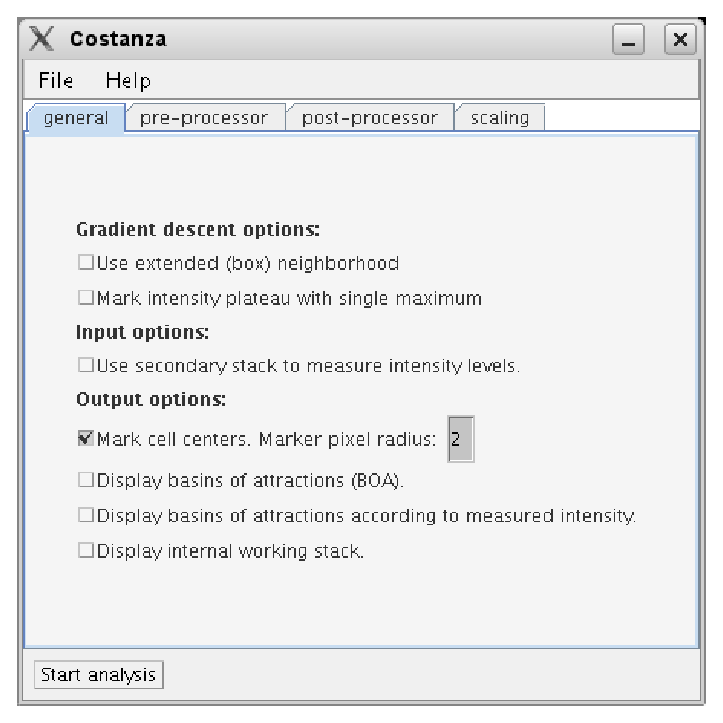
\includegraphics[width=0.49\columnwidth]{figures1/general.eps}
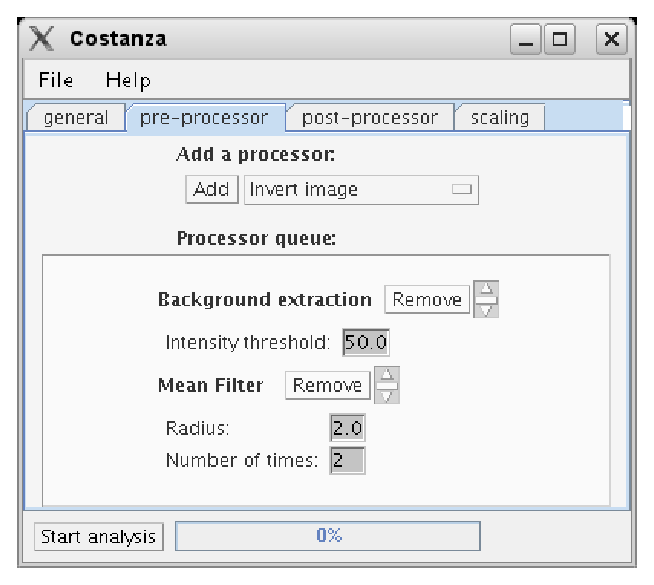
\includegraphics[width=0.49\columnwidth]{figures1/pre.eps}\\
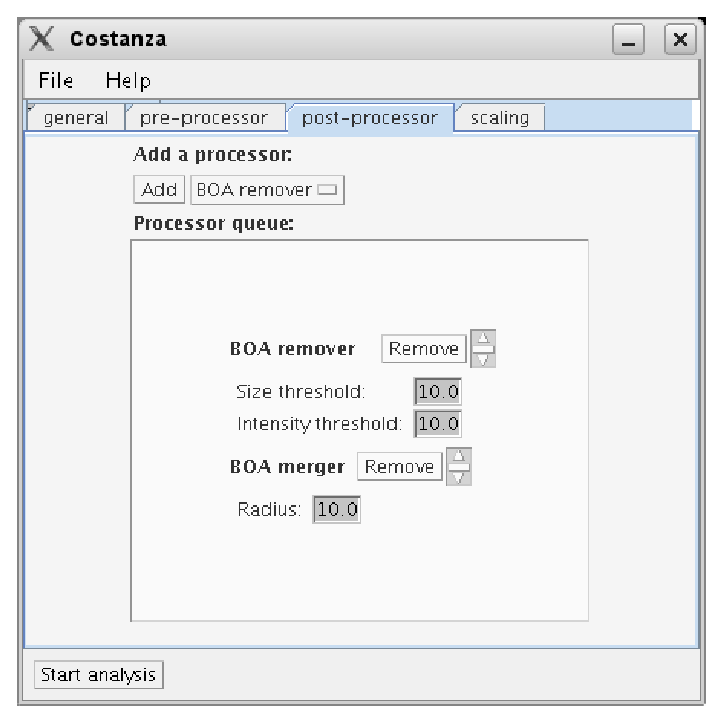
\includegraphics[width=0.49\columnwidth]{figures1/post.eps}
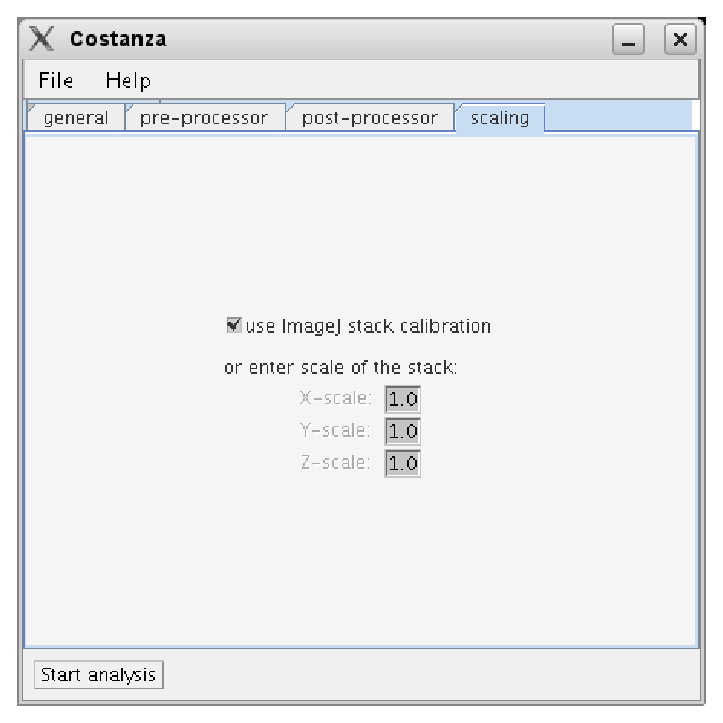
\includegraphics[width=0.49\columnwidth]{figures1/scaling.eps}
\caption{Graphical user interface for Costanza.}
\label{fig:gui}
\end{center}
\end{figure}
%

\subsubsection{General tab}
This tab allows for setting options for segmentation, gradient descent algorithm as well as input and output options. The active
stack is automatically chosen for segmentation input. If an additional stack is to
be used for measuring other intensities in previously found compartments, the box ``use secondary stack to measure intensity levels'' have to be checked.

As default, the segmentation results are provided in a table displayed by
ImageJ upon competition of analysis. Additionally other types of graphical output can be selected:

\begin{itemize}
%
\item Cell centers can be marked with red dots of desired radius in pixels.
%
\item Basin of Attractions (BOAs), attributed to the different cell centers can be
	colored with random colors.
%
\item BOAs can be colored and displayed according to measured intensities. The color schema is from blue via green yellow to red.
%
\item The working stack (after applying all the pre-processing options) can be displayed. This can be useful to see how the
	pre-processing has changed the original images.
%
\end{itemize}

\subsubsection{Pre-processing}
Here different pre-processing steps can be chosen, added and removed by the
user. Processors in the queue will be applied to the stack in top to bottom order. The alternatives at the moment are:

\begin{itemize}
%
\item Invert - inverts the pixels in the stack. This is needed if the objects
	are dark in a brighter background, \textit{e.g.} if bright membranes are marking
	cells.
%
\item Background threshold - this will put all pixels below a threshold
	intensity to the background, and hence they will not be processed by other algorithms and 
	the segmentation in particular.
%
\item Mean Filter - this will reduce noise in the images by applying a 3D mean
	filter with provided radius. As it is often useful to apply this more than
	once, repeat option is also provided for the user.
%
\item Median Filter - another alternative to reduce image noise is to apply 3D median filter.
	Radius and repeat options are available to set by the user as in previous case.
%
\end{itemize}

\subsubsection{Post-processing}
After the gradient descent algorithm is applied for segmentation, it might be
useful to do some post-processing. As previously order of application of processors is from top to bottom. The available algorithms that can be chosen, added and removed are:

\begin{itemize} 
%
\item BOA remover, where BOA regions attributed to compartments can be removed due to being too small
	or having too low intensity.
%
\item BOA merger, where compartments with centers too close to each other can be
	merged into a single compartment.
%
\end{itemize}

\section{Examples}
The performance of the Costanza application is dependent on the
parameter values given to the different algorithms used. This values will be most likely different for different tasks or even set of images. Thus getting satisfactory results in each case may require some experimenting and tweaking different parameters. Here we provide
some examples of applications where also the parameter values used are
presented to guide users into setting reasonable parameter values.

\subsection{SAM nuclei data in 3D}
This data set represents nuclei marked cells in the Arabidopsis shoot apical
meristem. The data set consists of a stack of 20 images. For simplicity and readability reasons we present results of analysis of single 2D slice from the stack but the whole 3D stack can be processed equaly well. The
segmentation is run using two different resolutions, and the result is shown in Fig.~\ref{fig:43zoom}. Parameters used for these two runs are given in Table~\ref{tab:43zoom}, and should represent reasonable values also for 3D stacks.
\begin{figure}[h!]
\begin{center}
\subfloat[100x100 pixels image]{
\label{fig:small43centers}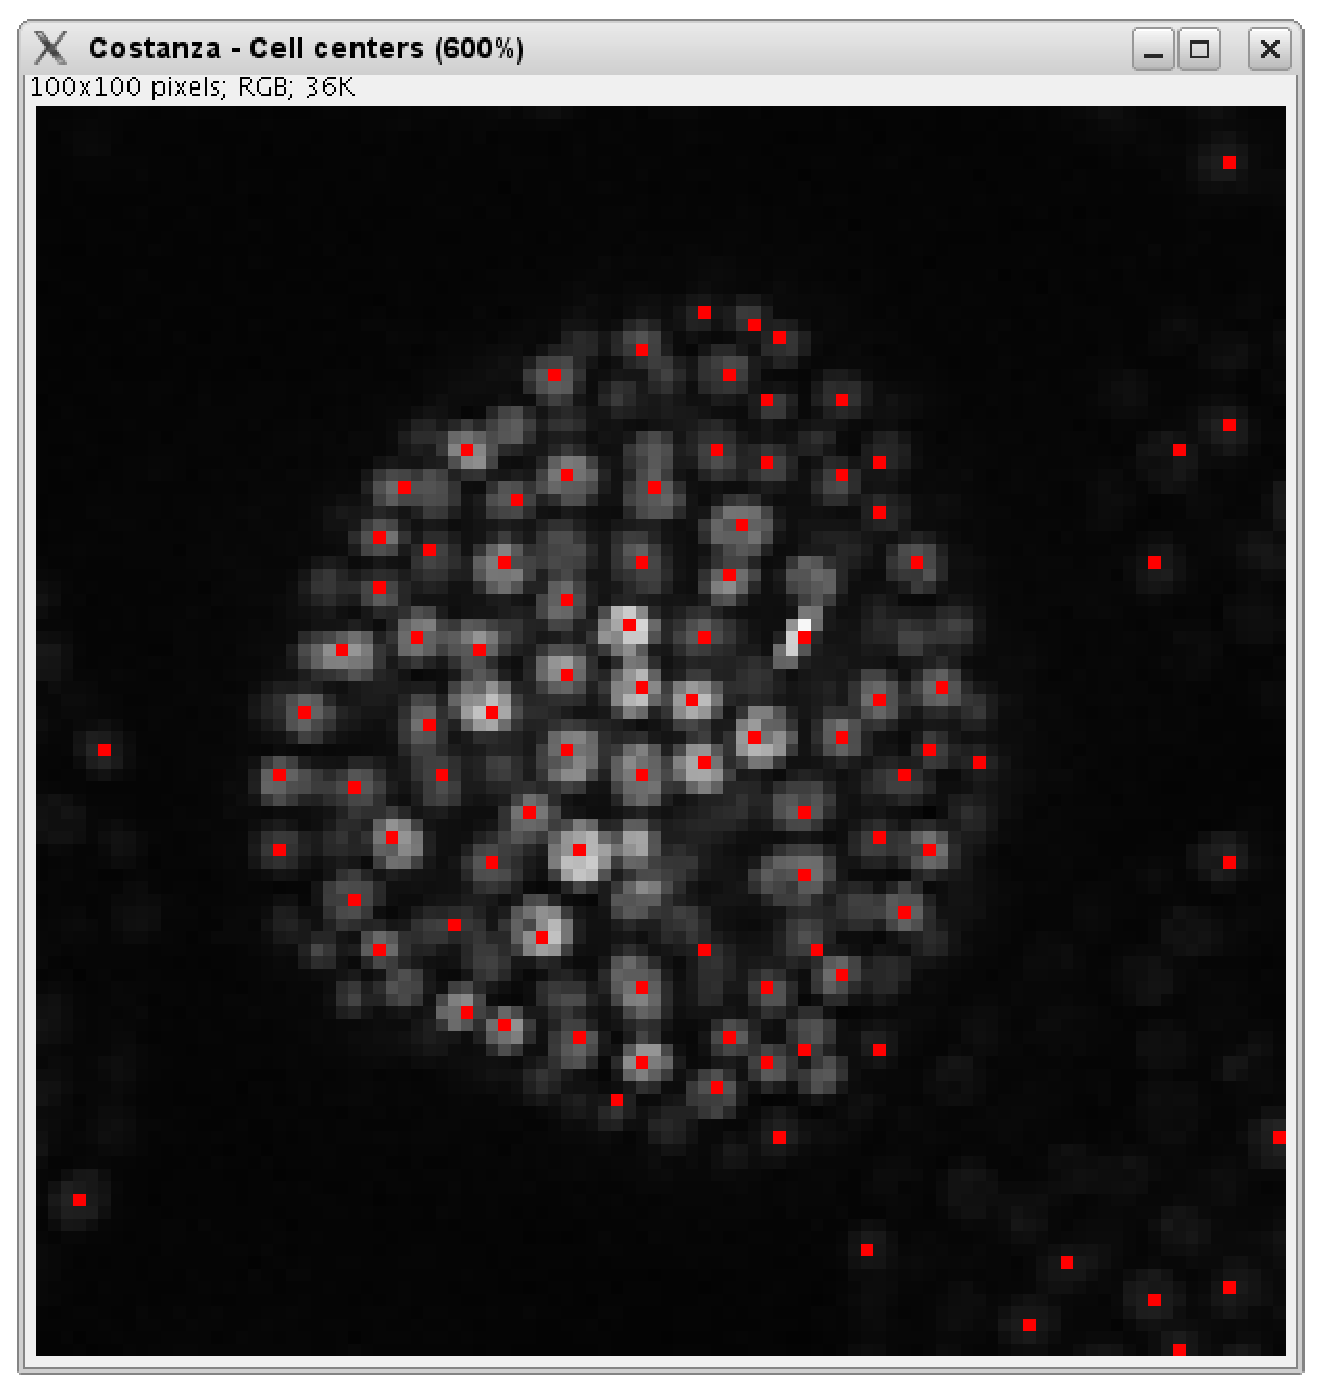
\includegraphics[width=0.4\columnwidth]{figures1/centers_small.eps}
\label{fig:small43boas}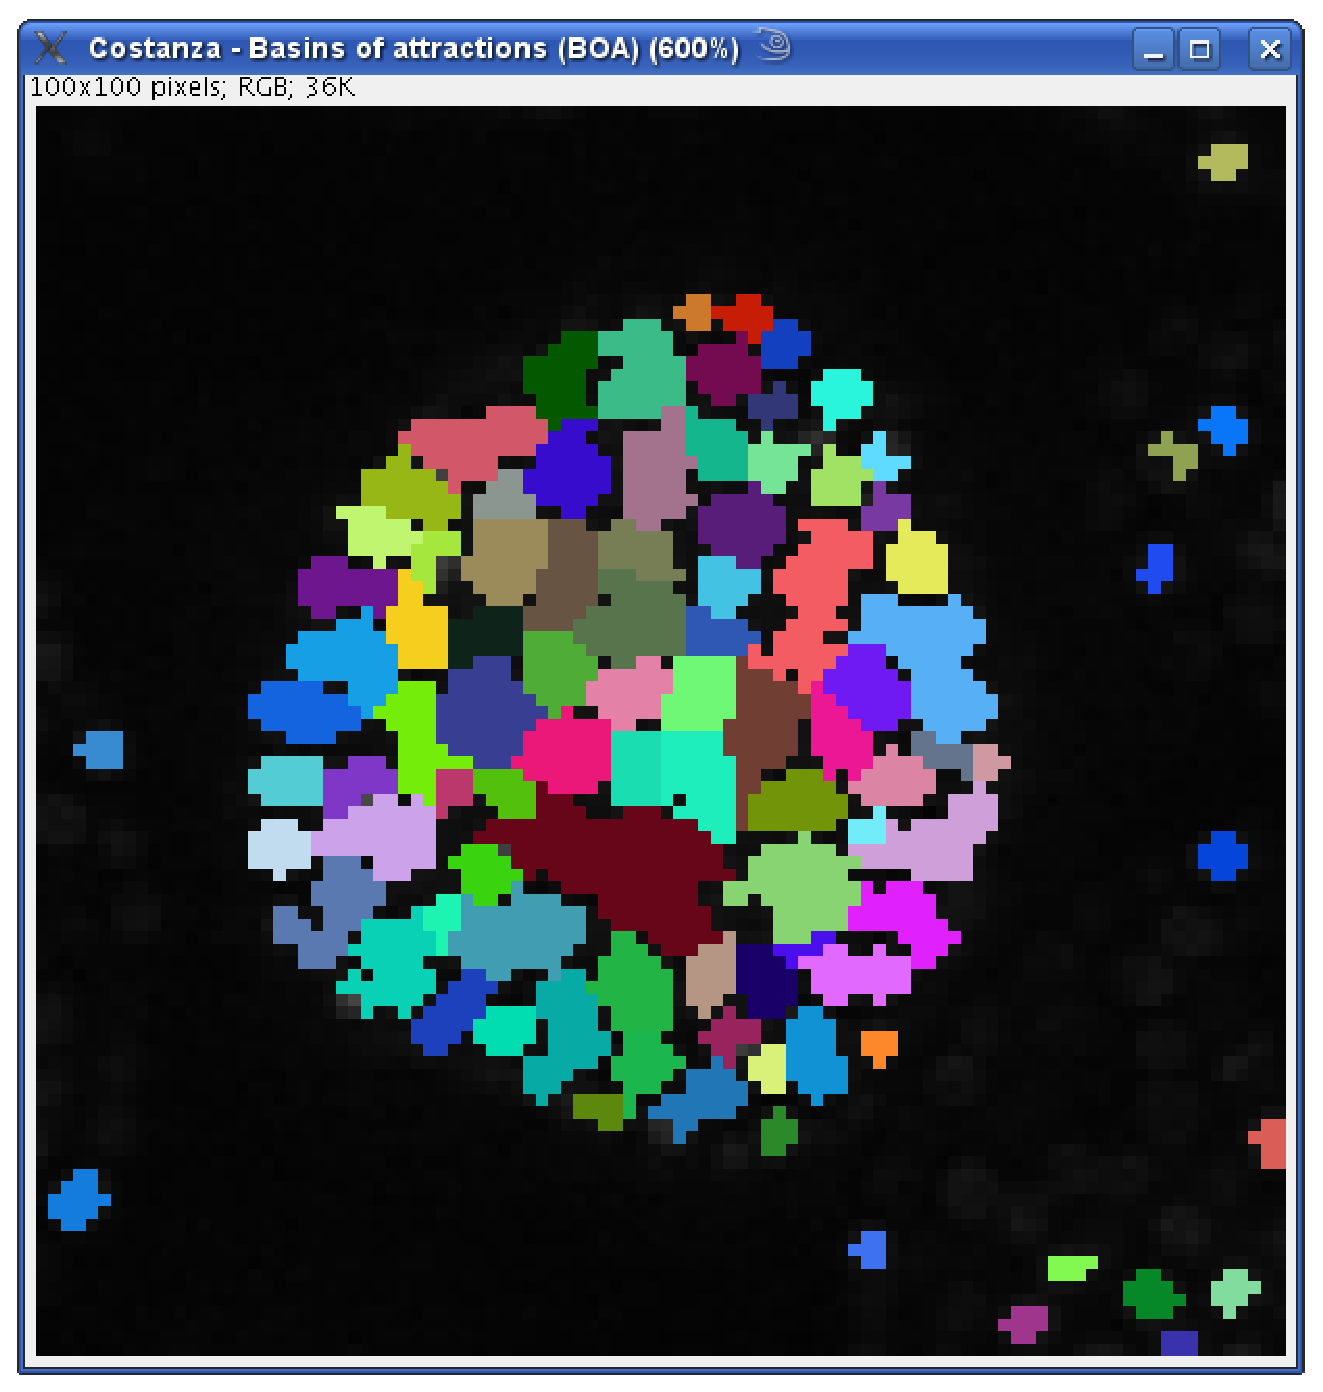
\includegraphics[width=0.4\columnwidth]{figures1/boas_small.eps}
}\\
\subfloat[512x512 pixels image]{
\label{fig:43centers}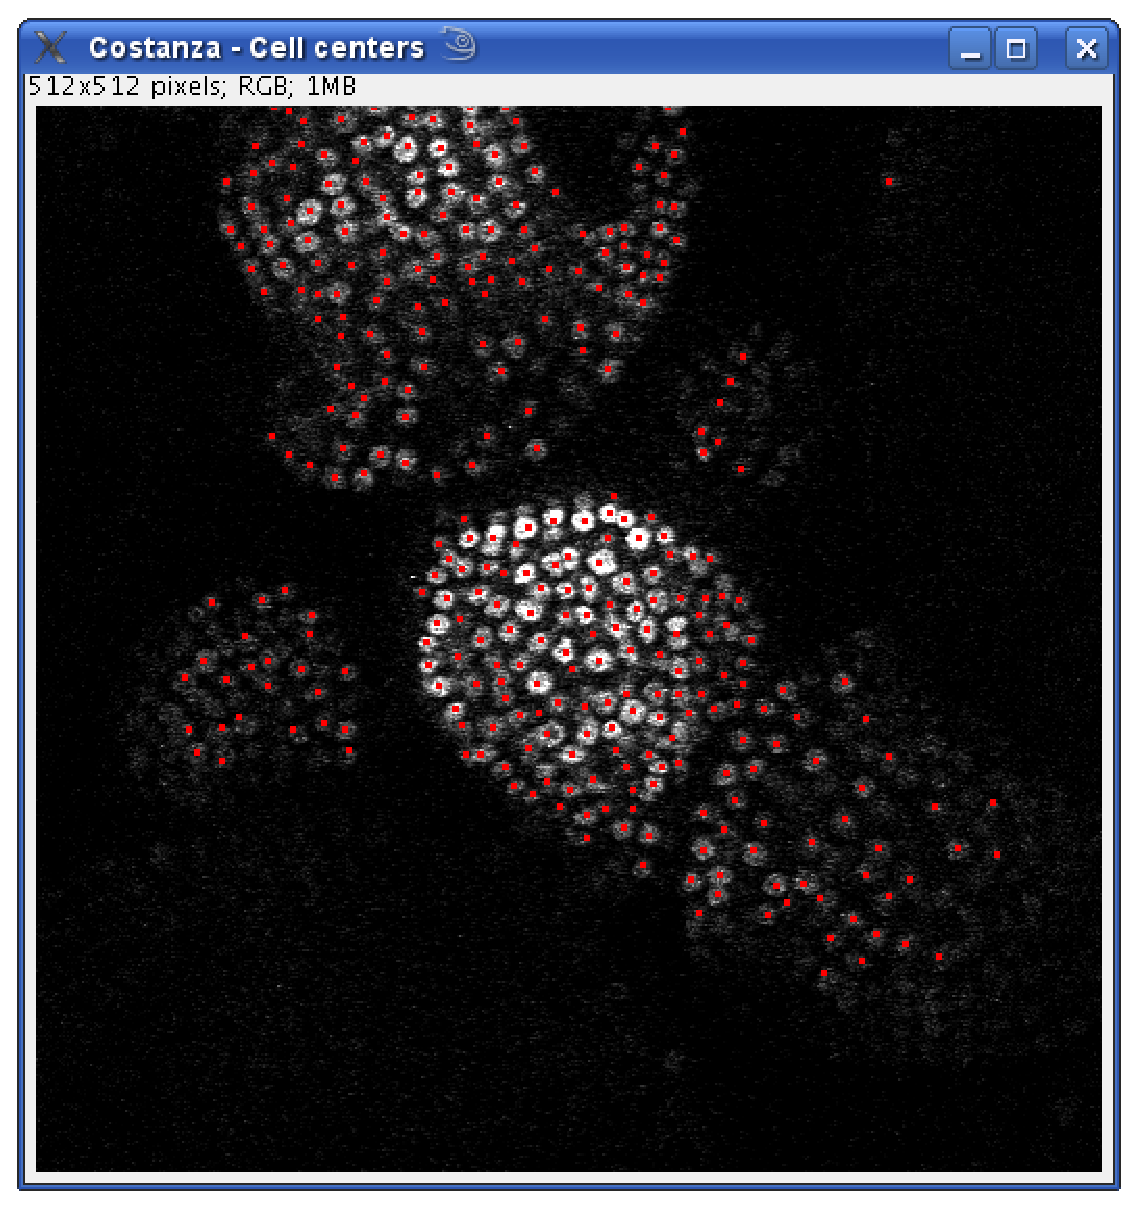
\includegraphics[width=0.4\columnwidth]{figures1/centers.eps}
\label{fig:43boas}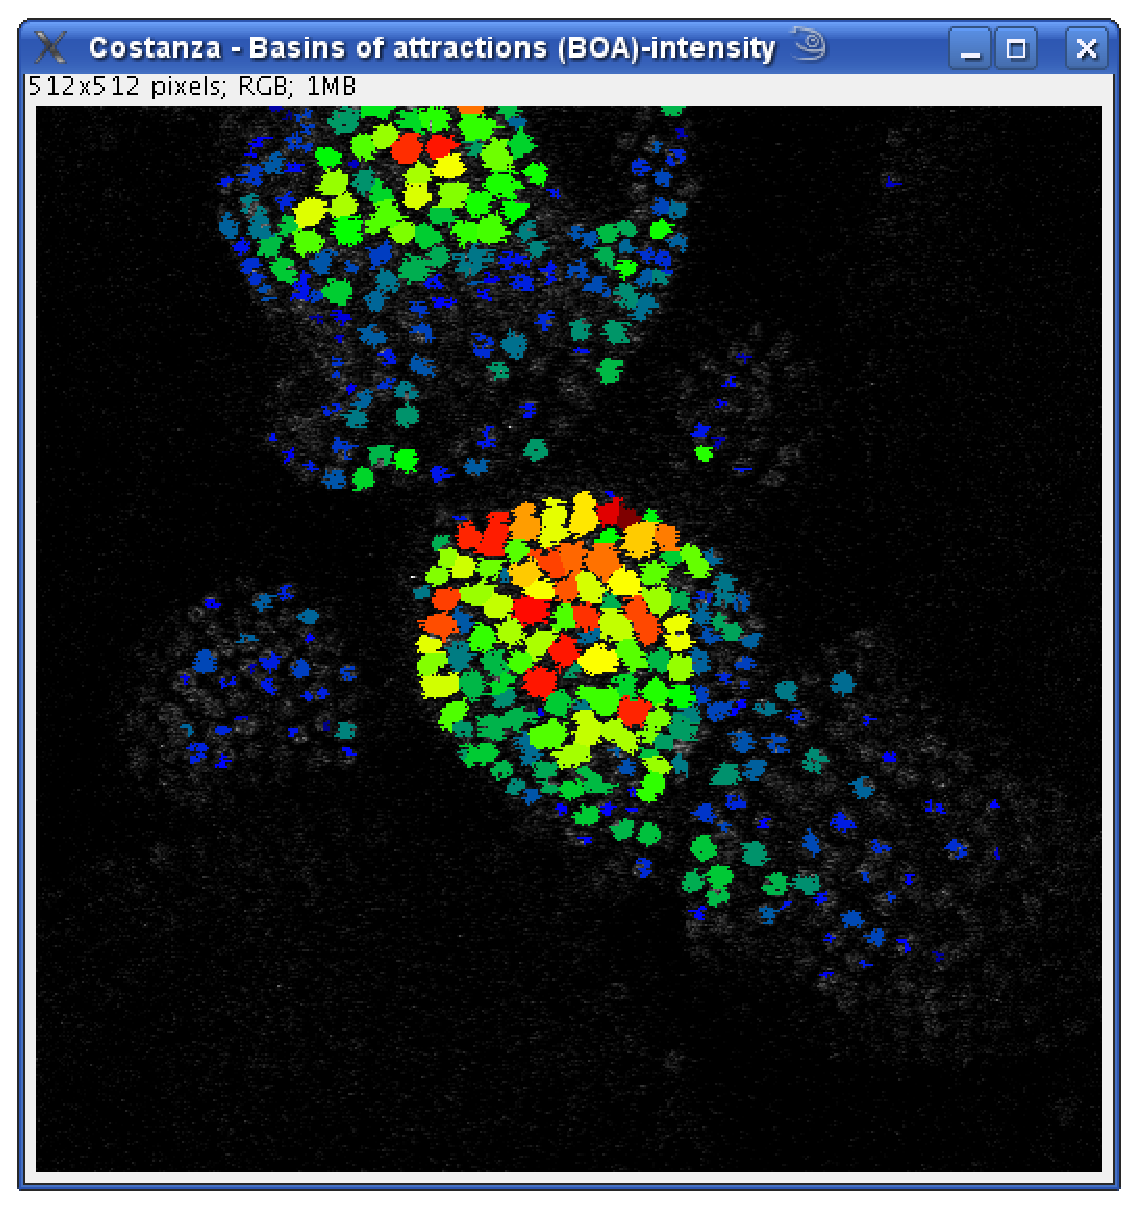
\includegraphics[width=0.4\columnwidth]{figures1/boas.eps}
}
\caption{Result shown for images of nuclei data. Original images can be found at http://www.thep.lu.se/...}
\label{fig:43zoom}
\end{center}
\end{figure}


\begin{table}
	\begin{center}
		\begin{tabular}{|l|cc|}
			\hline
			Parameter & Small & Large\\
			\hline
			Bg threshold & 20 & 30\\
			MeanFilter R & 1.0 & 2.0\\
			MeanFilter num & 2 & 2\\
			Remove Int Th. & 6 & 10\\
			Remove Size Th. & 6 & 10\\
			Merger R & 3 & 7\\
			xy-scale & 1 & 1\\
			z-scale & 1 & 1\\
			\hline
		\end{tabular}
		\caption{Nuclei extraction in 2D and 3D.}
		\label{tab:43zoom}
	\end{center}
\end{table}

\subsection{SAM membrane data in 2D}


This data set represents membrane marked cells in the Arabidopsis shoot apical
meristem. The data set consists of single 2D images. The segmentation is run
using two different resolutions, and the result is shown in
Fig.~\ref{fig:membrane}.

\begin{figure}[h!]
\begin{center}
\label{fig:memebraneA1}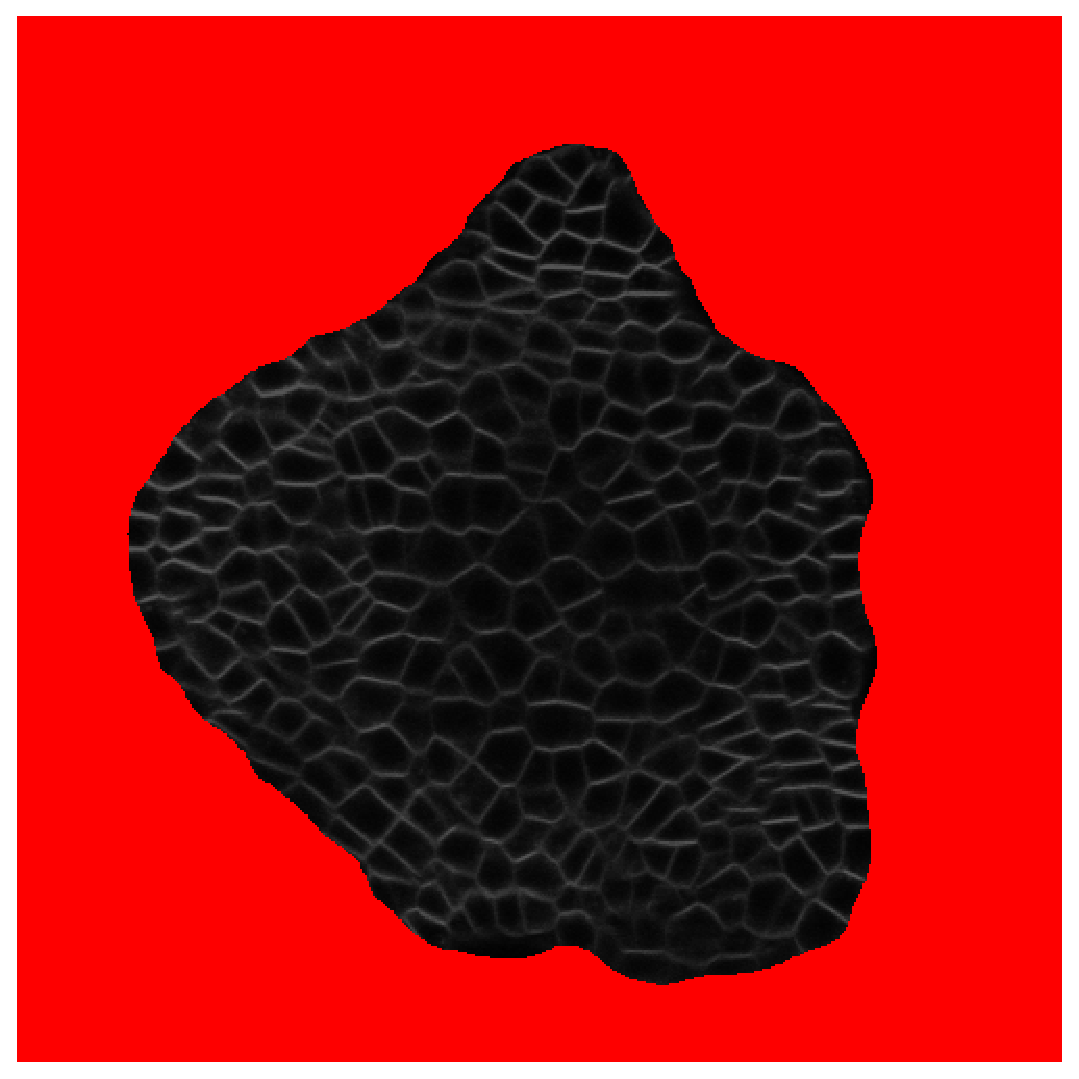
\includegraphics[width=0.25\columnwidth]{figures/wusMembrane.eps}
\label{fig:memebraneA2}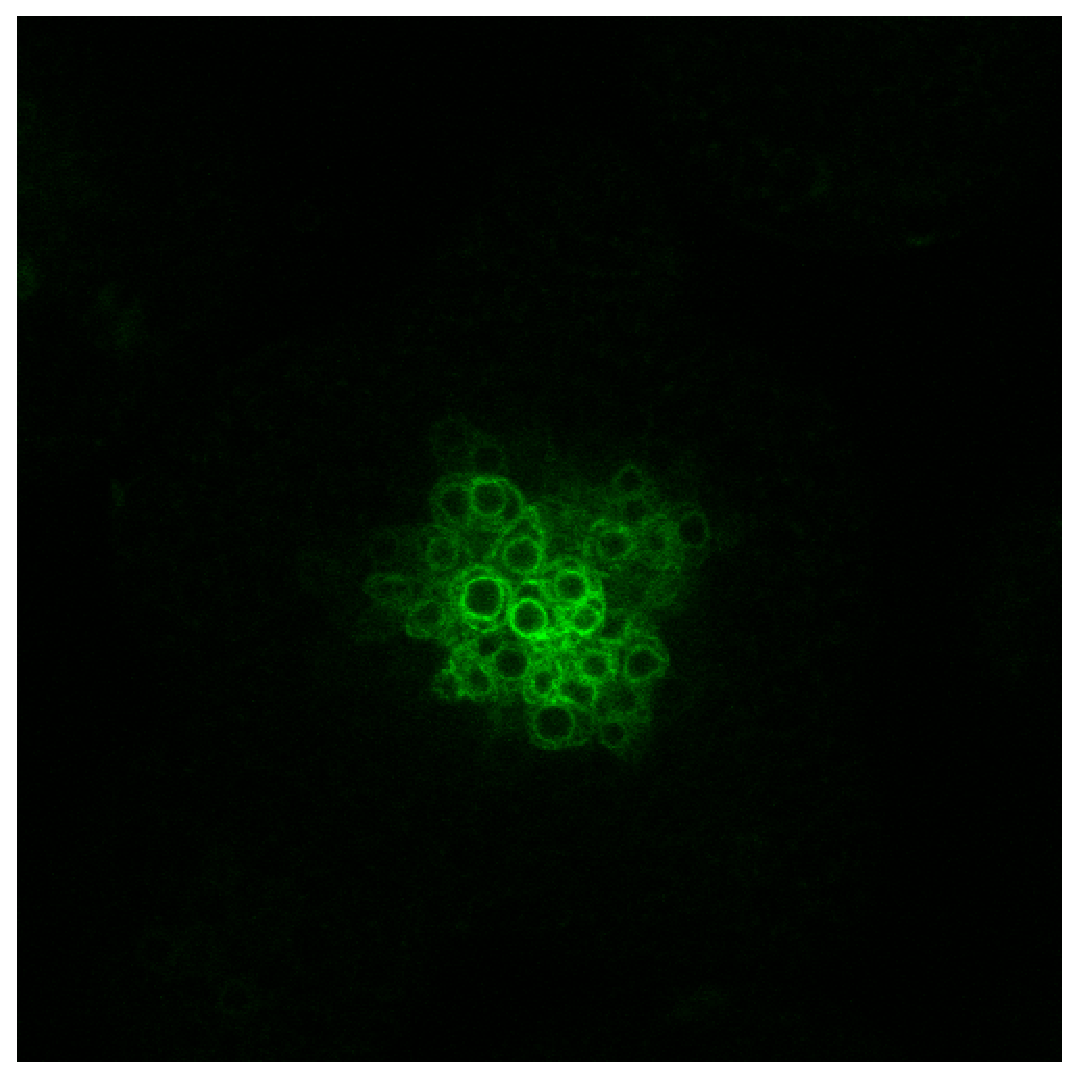
\includegraphics[width=0.25\columnwidth]{figures/wusWus.eps}\\
\label{fig:memebraneA3}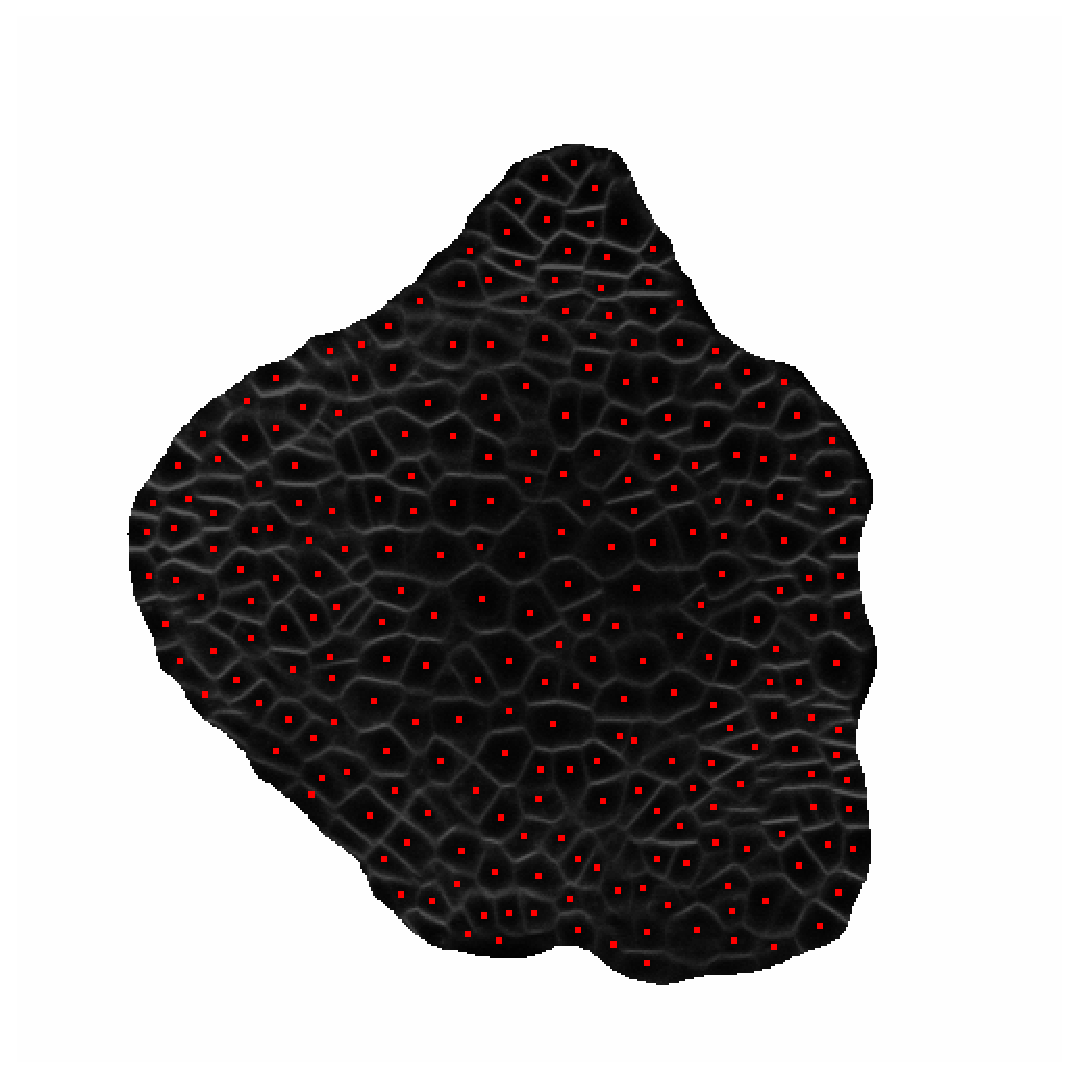
\includegraphics[width=0.25\columnwidth]{figures/wusCenters.eps}
\label{fig:memebraneA4}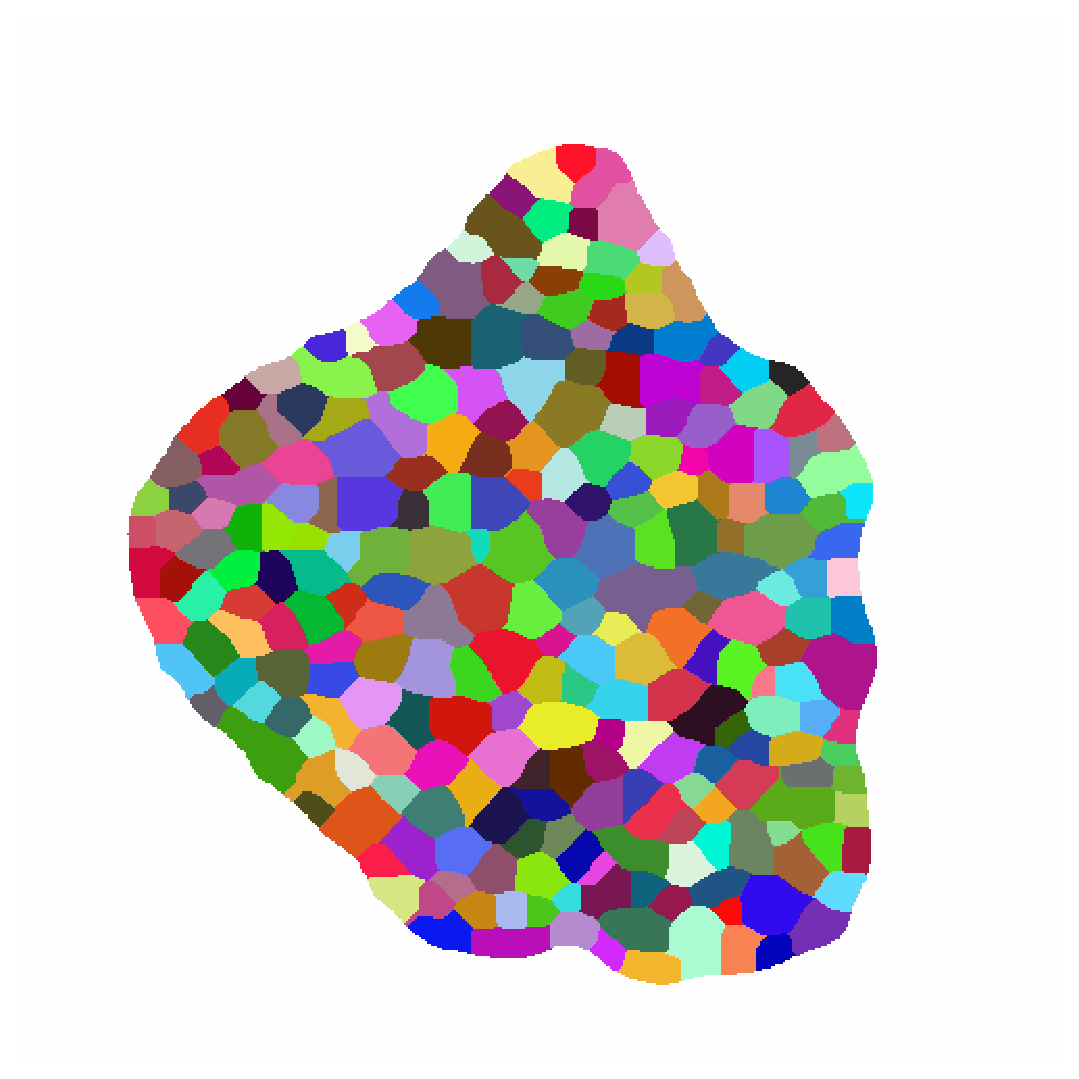
\includegraphics[width=0.25\columnwidth]{figures/wusBOAs.eps}
\label{fig:memebraneA5}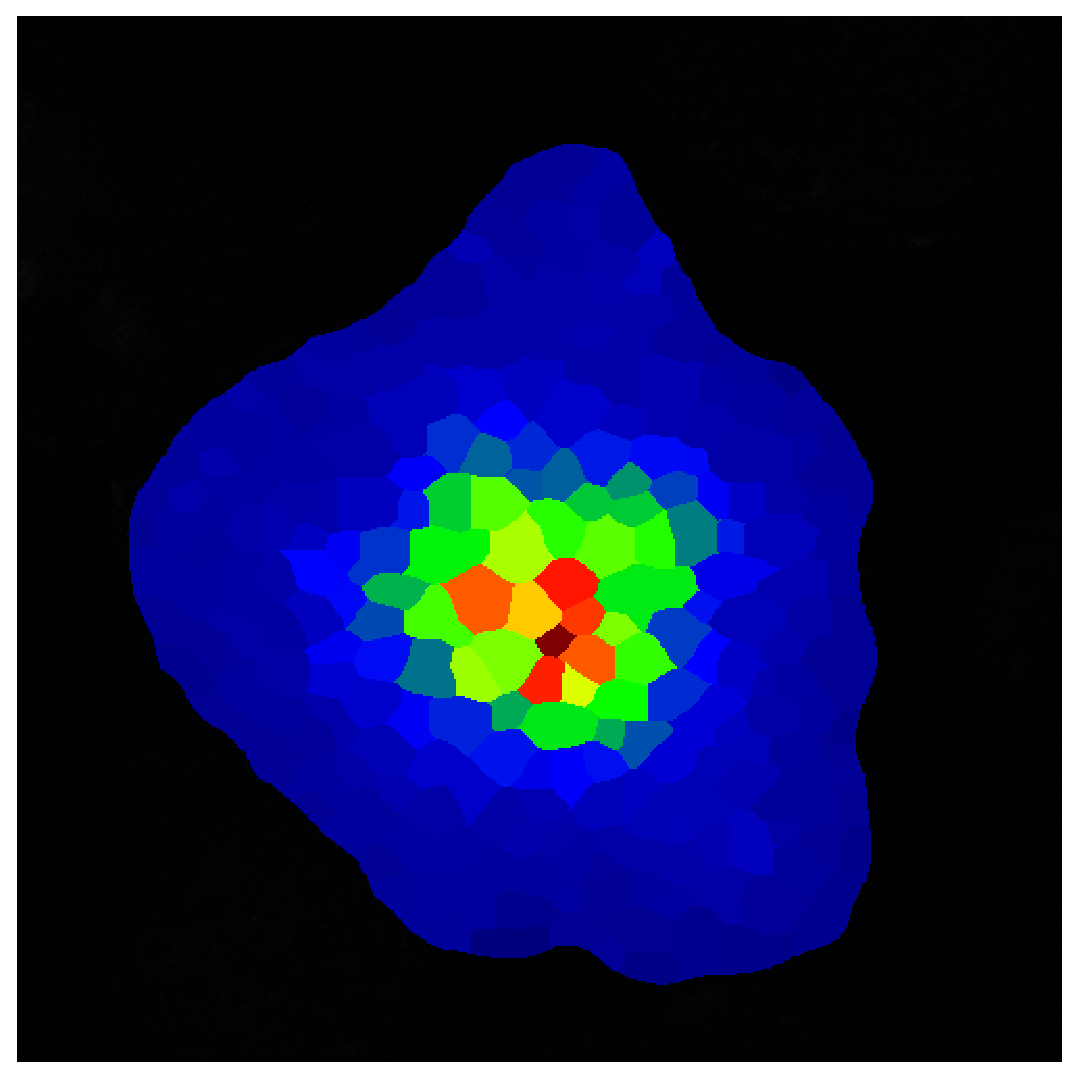
\includegraphics[width=0.25\columnwidth]{figures/wusBOAsIntensity.eps}
\vspace{4 mm}
\label{fig:memebraneB1}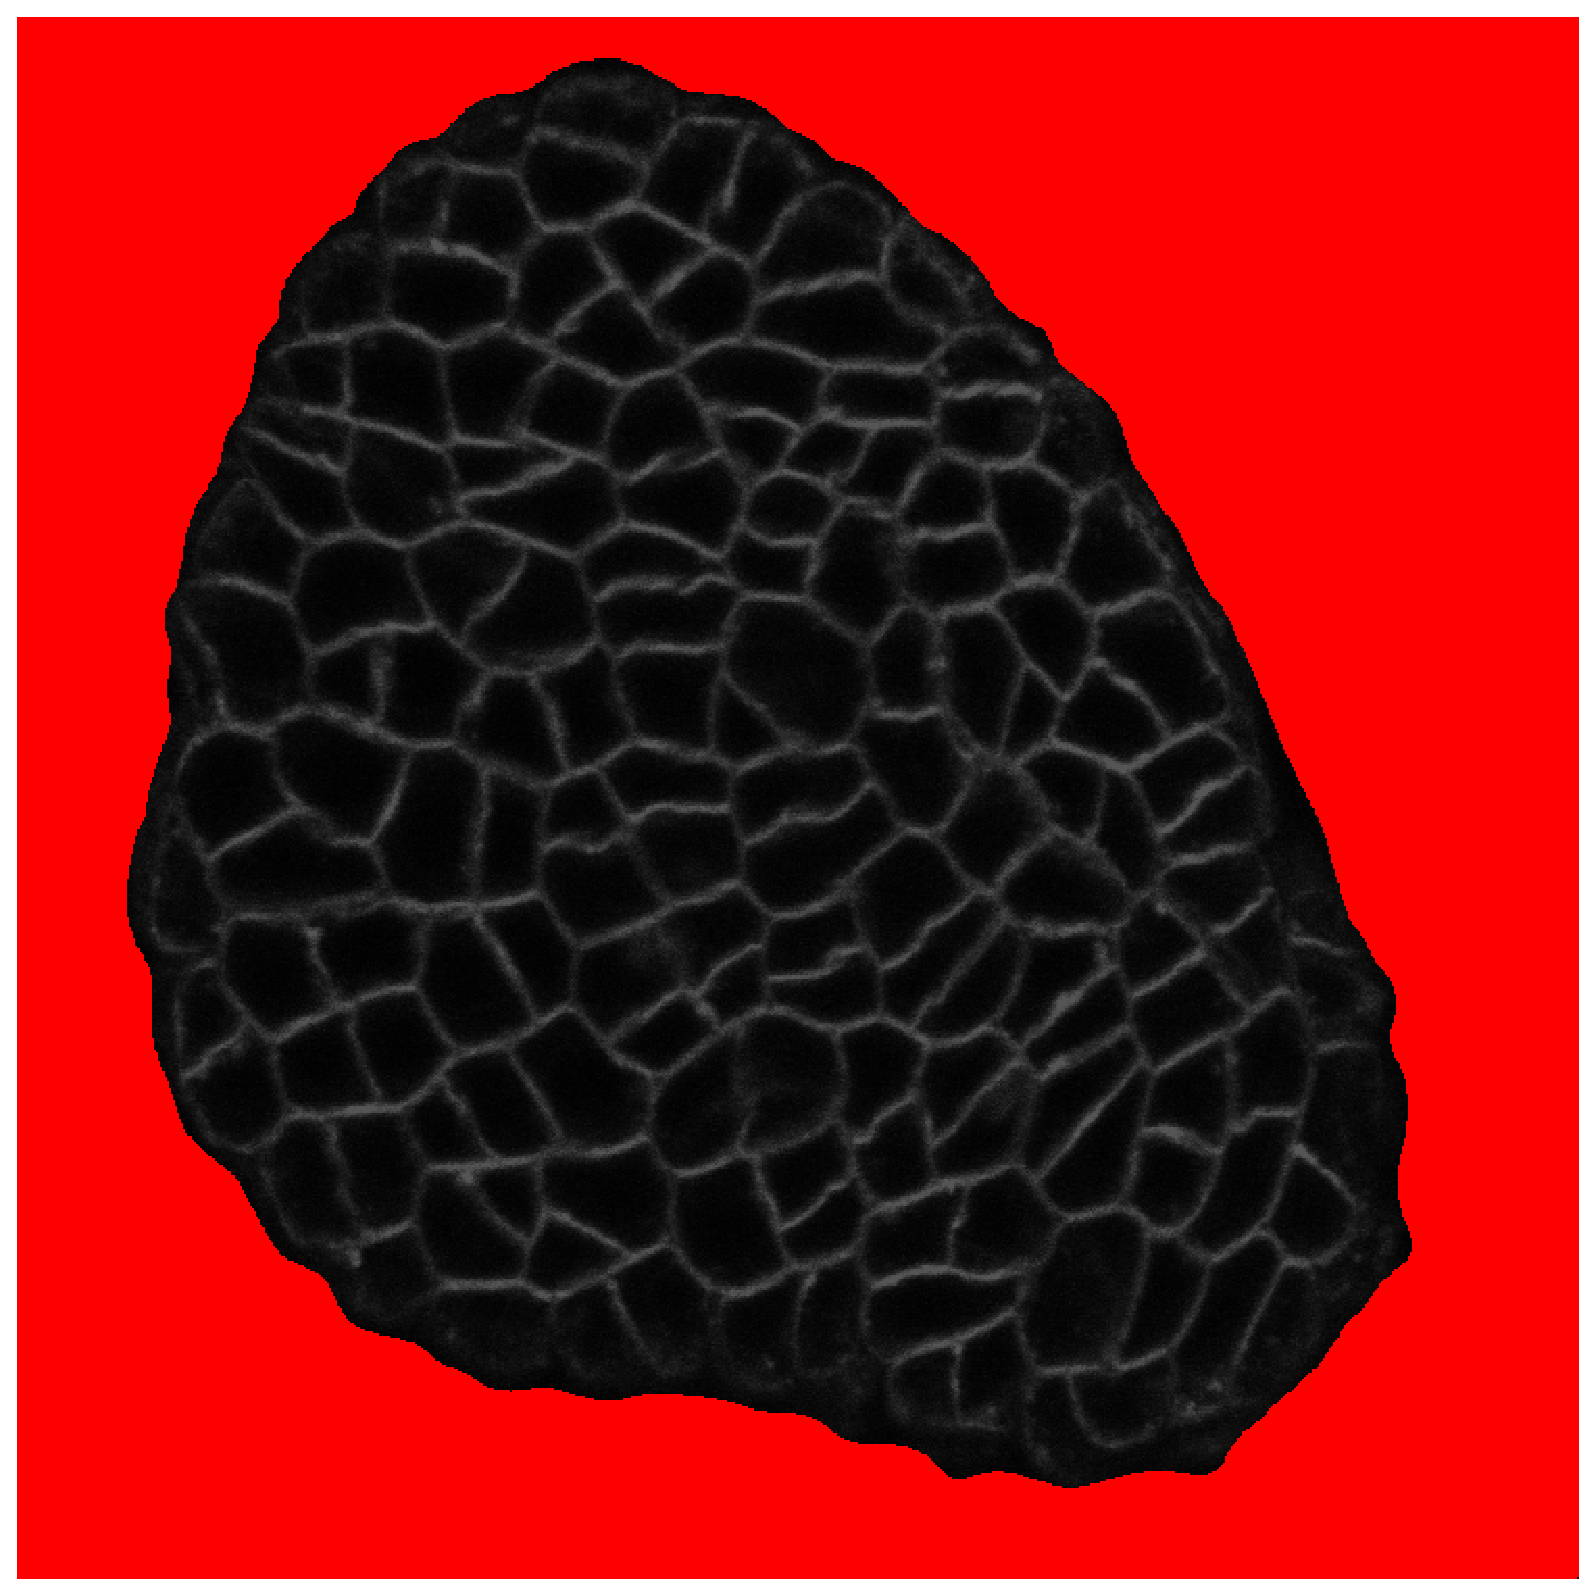
\includegraphics[width=0.33\columnwidth]{figures/pin1Membrane.eps}
\label{fig:memebraneB2}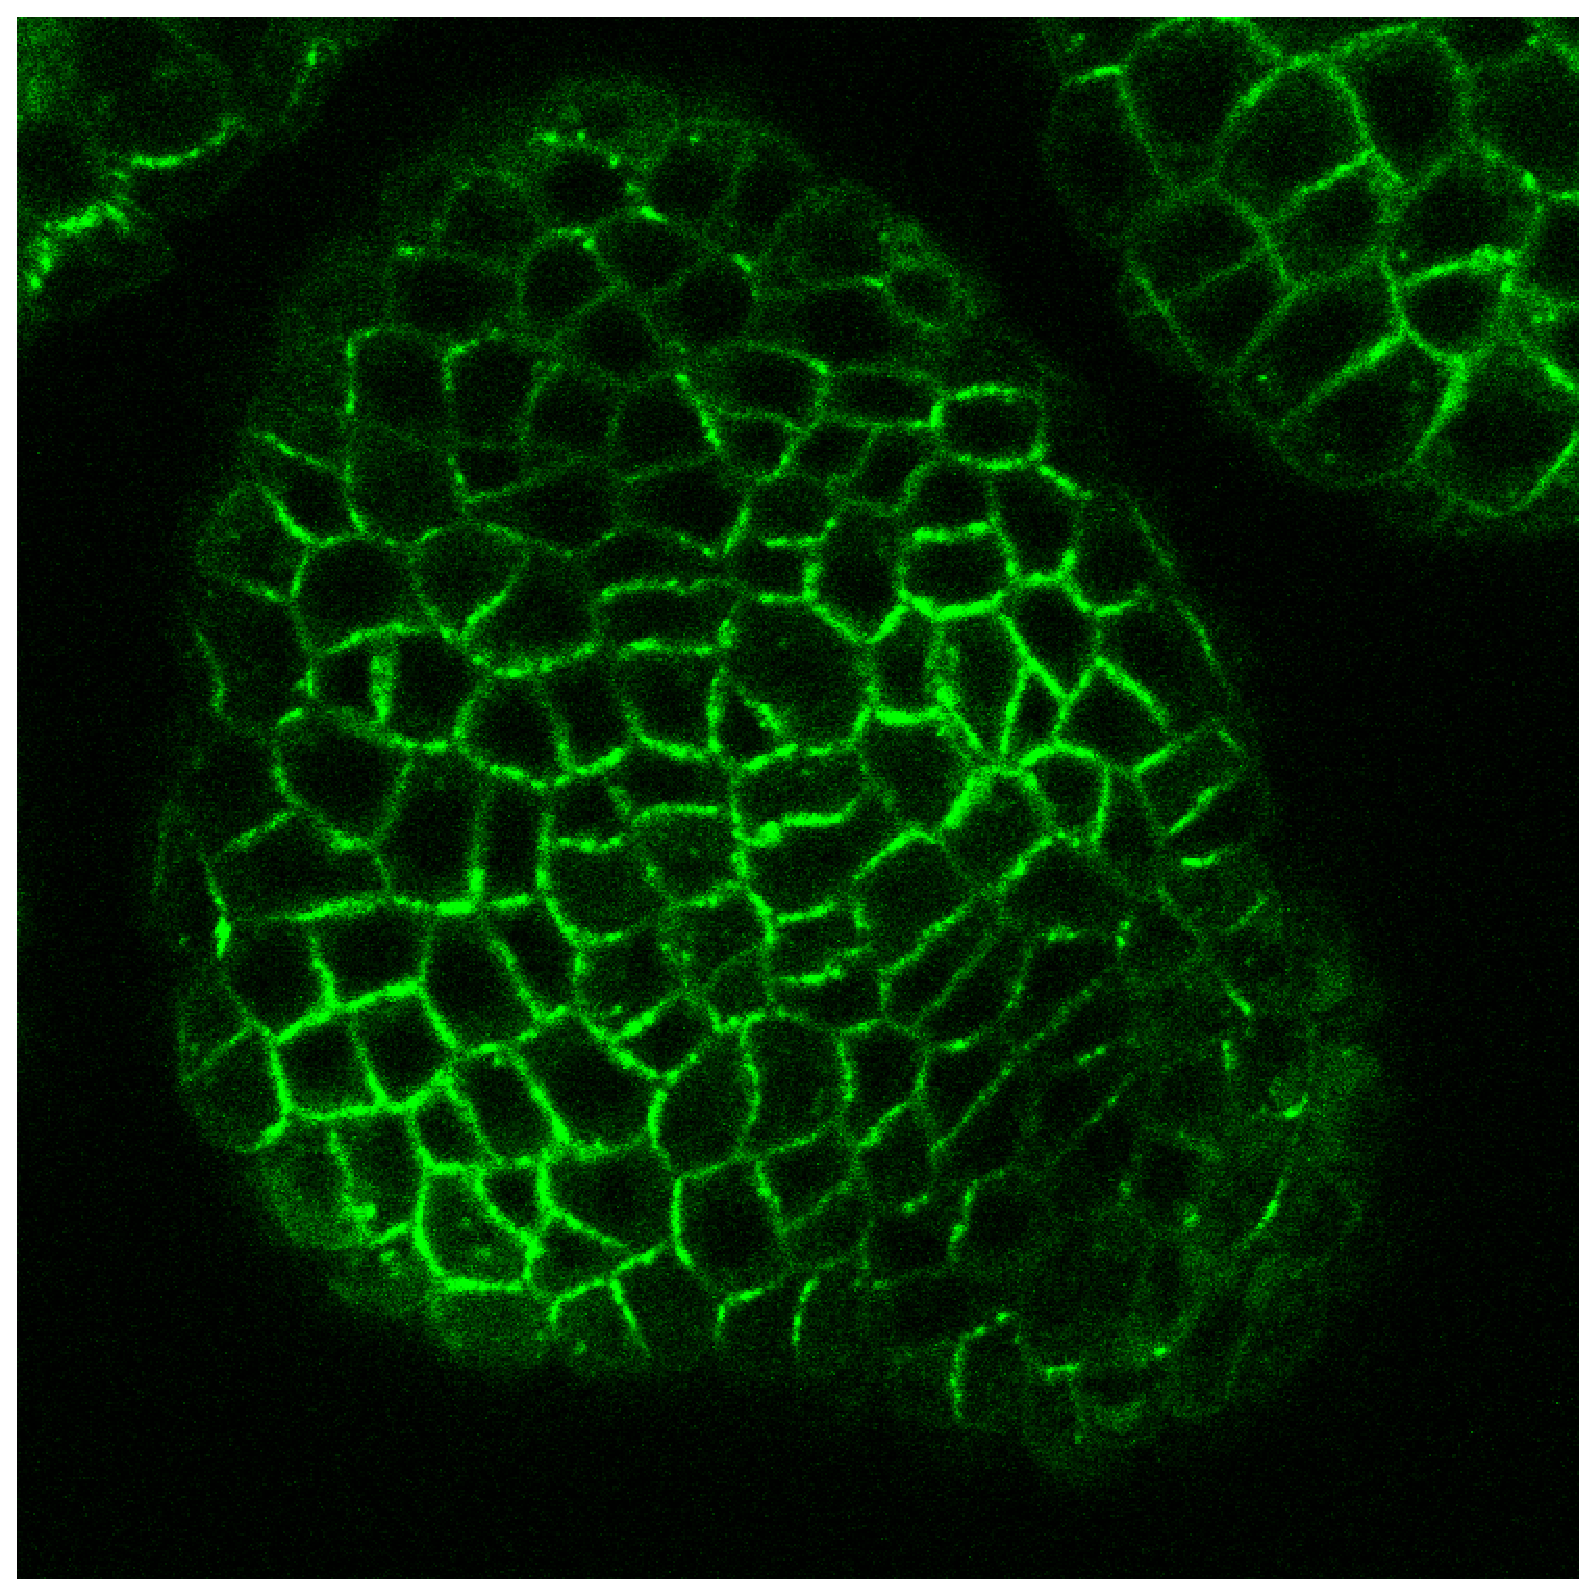
\includegraphics[width=0.33\columnwidth]{figures/pin1Pin1.eps}\\
\label{fig:memebraneB3}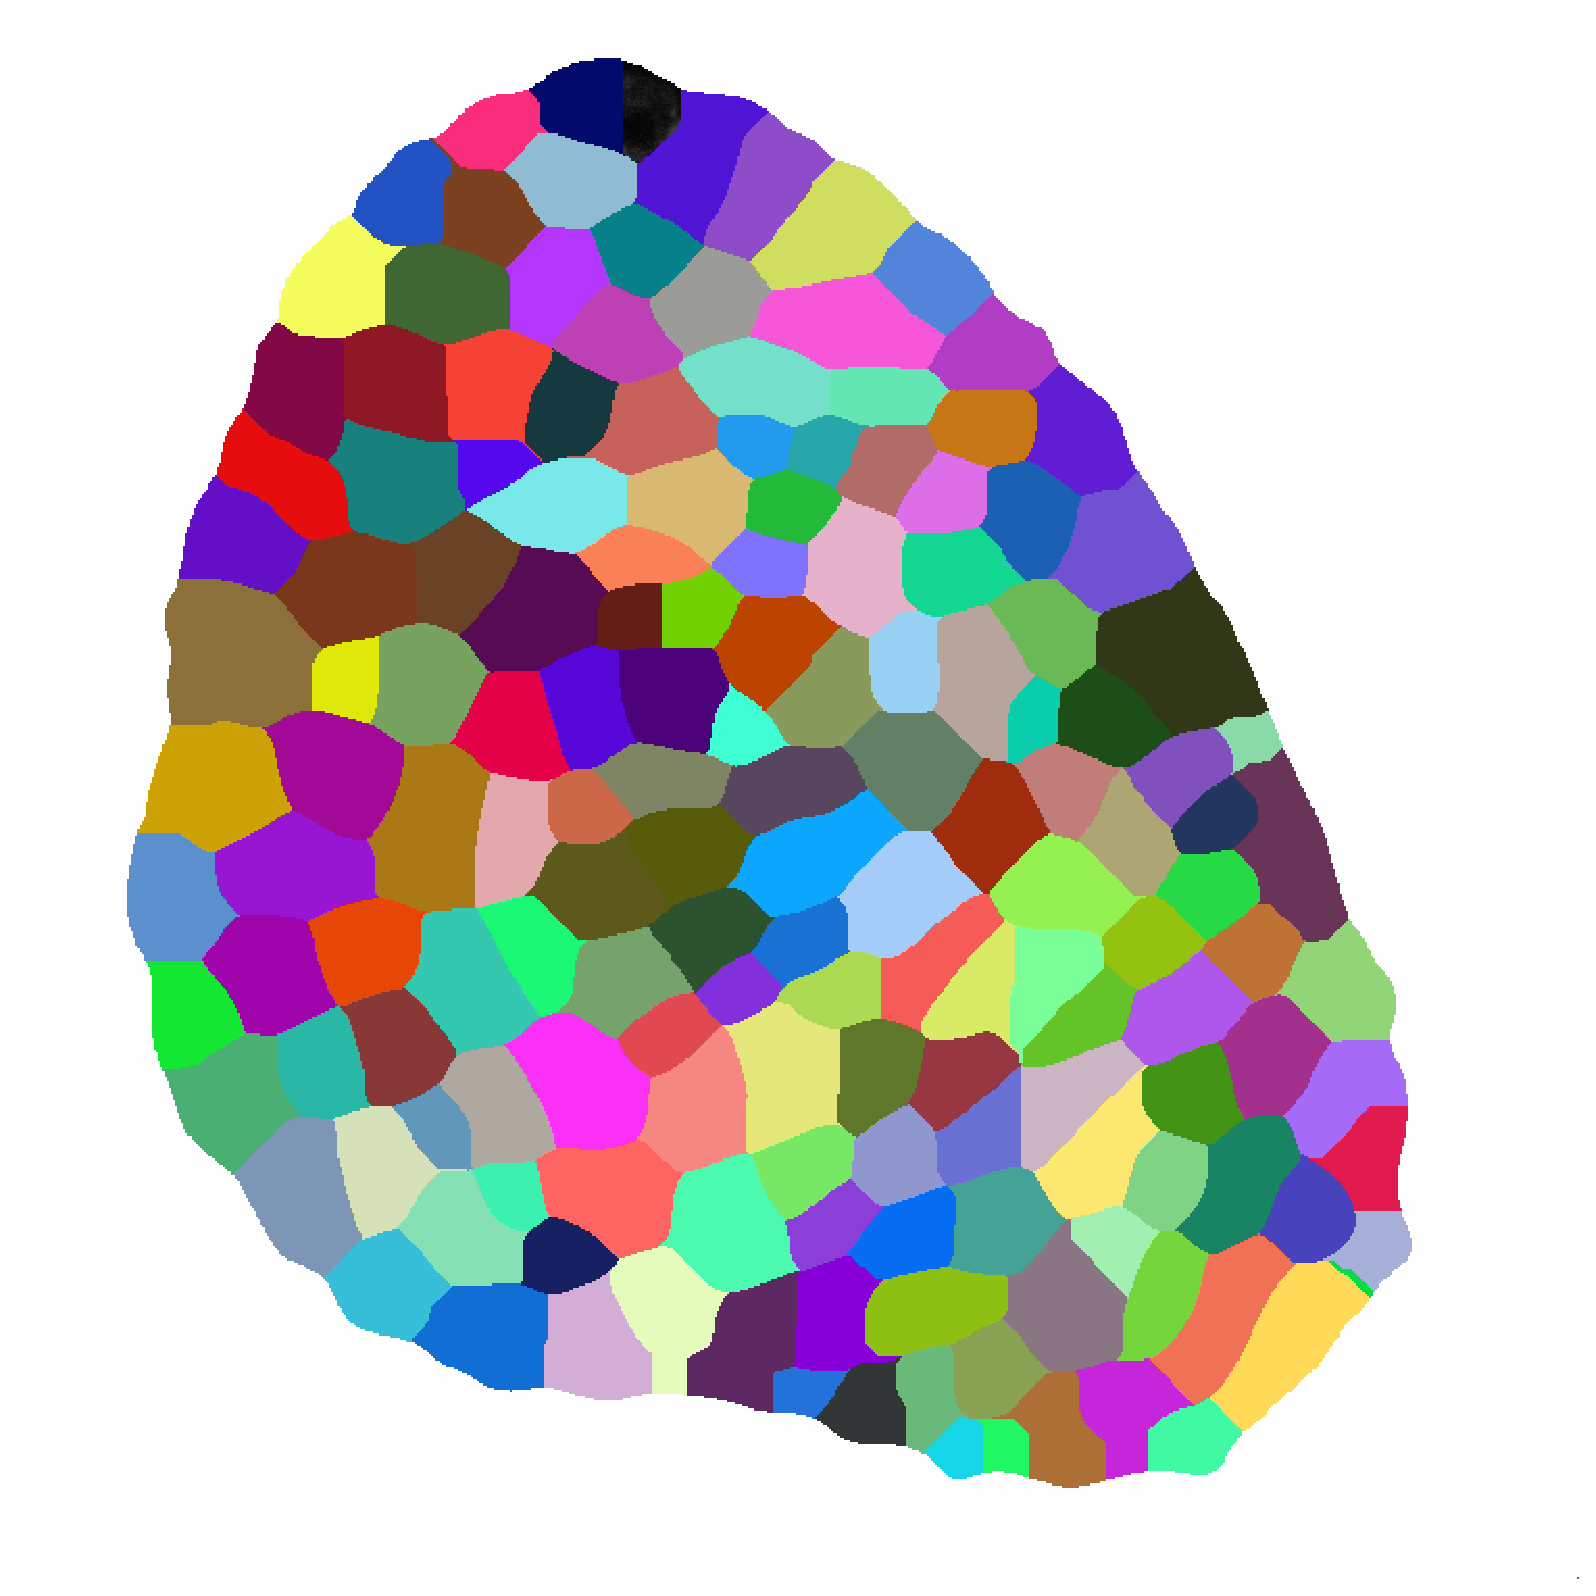
\includegraphics[width=0.33\columnwidth]{figures/pin1BOAs.eps}
\label{fig:memebraneB4}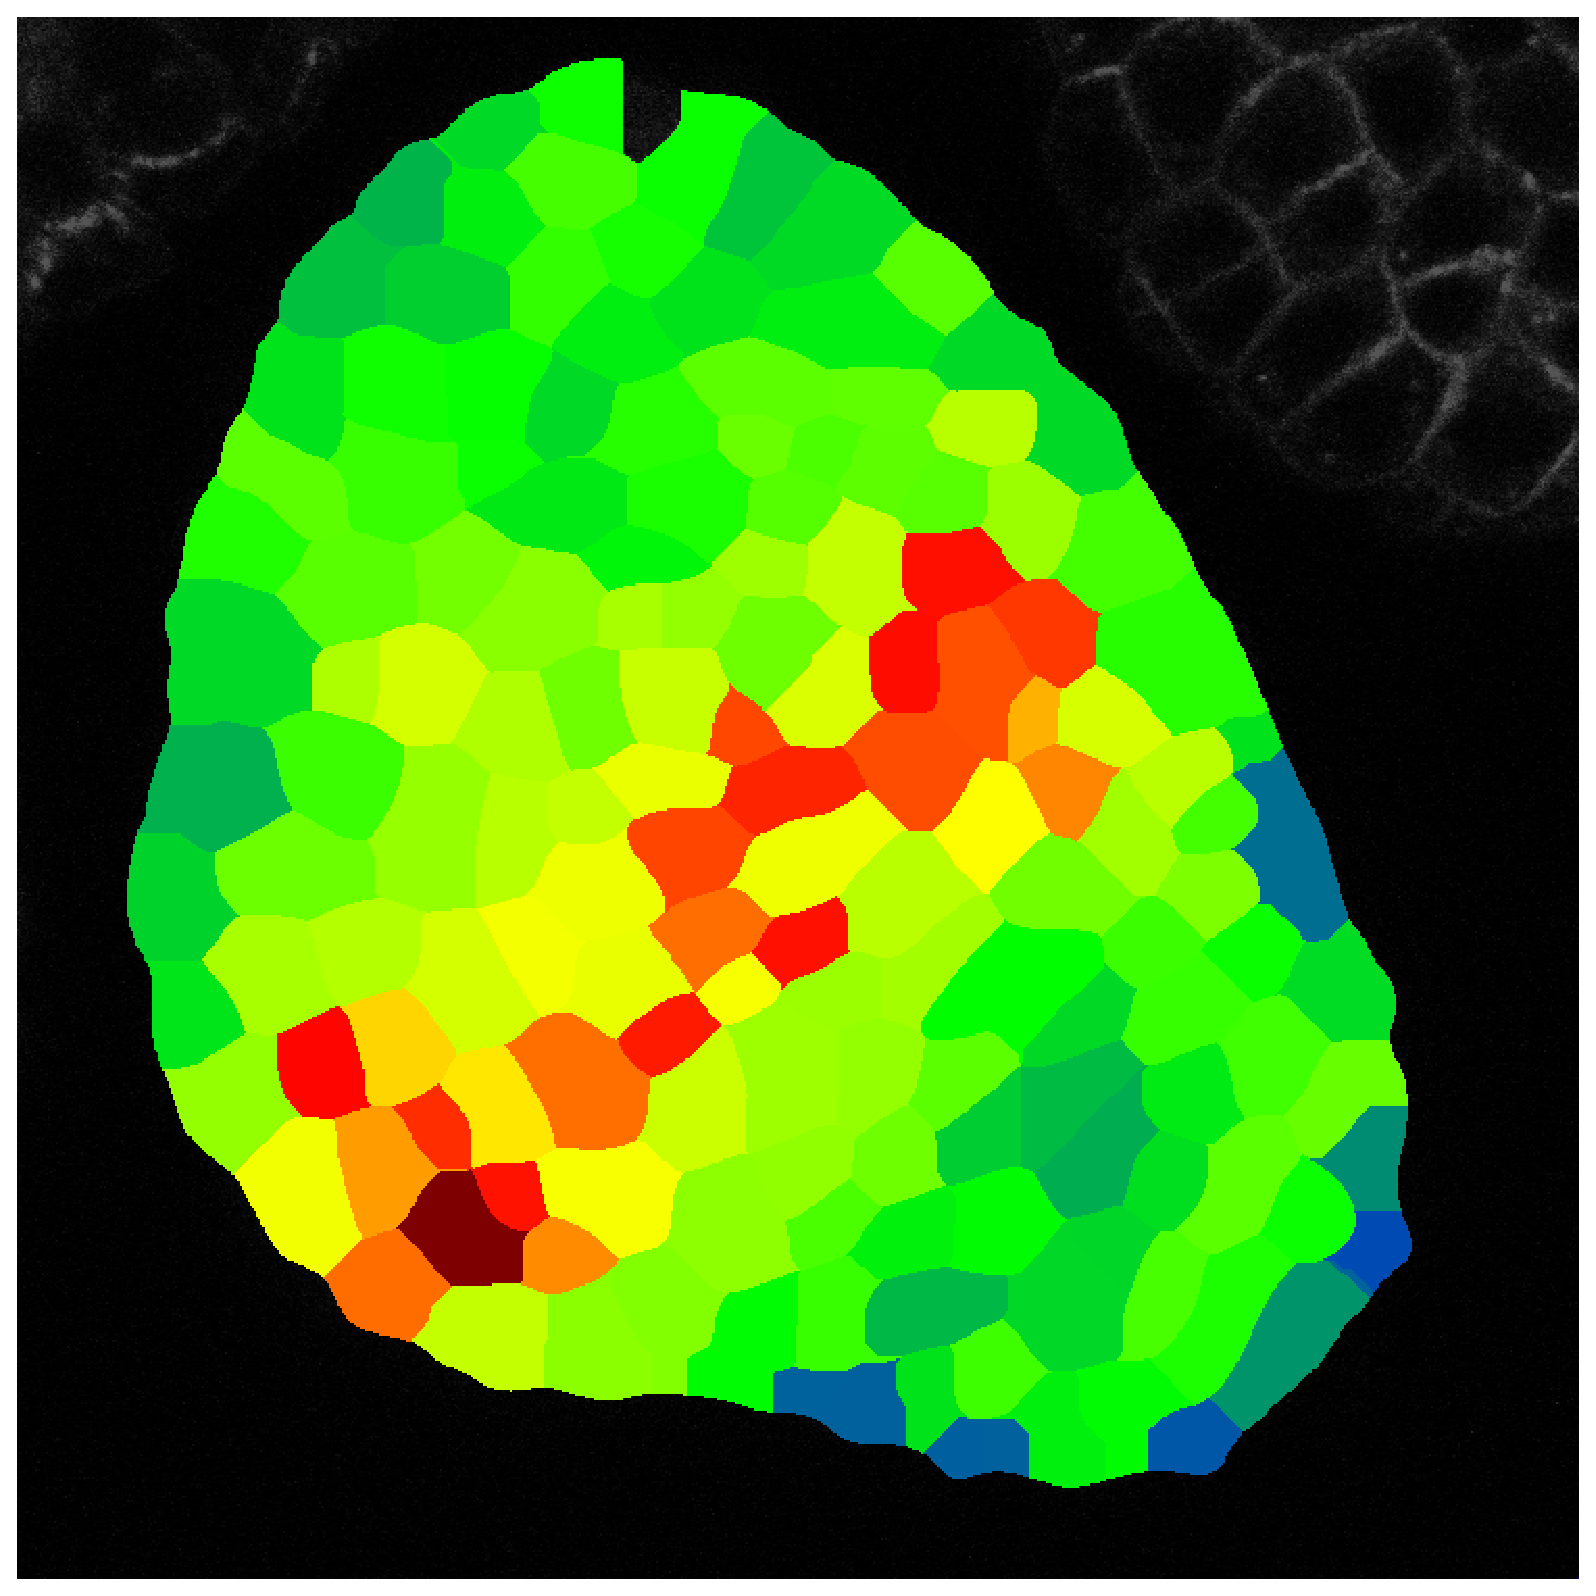
\includegraphics[width=0.33\columnwidth]{figures/pin1BOAsIntensity.eps}
\caption{Result shown for images of membrane data. Original images can be
	found at http://www.thep.lu.se/...}
\label{fig:membrane}
\end{center}
\end{figure}
%
Parameters used for these two segmentations are given in Table~\ref{tab:membrane}.

\begin{table}
	\begin{center}
		\begin{tabular}{|l|cc|}
			\hline
			Parameter & WUS & PIN1\\
			\hline
			Bg threshold & 1 & 1\\
			MeanFilter R & 5.0 & 10.0\\
			MeanFilter num & 2 & 2\\
			Remove Int Th. & 10 & 10\\
			Remove Size Th. & 10 & 10\\
			Merger R & 5 & 10\\
			xy-scale & 1 & 1\\
			z-scale & - & -\\
			\hline
		\end{tabular}
		\caption{Cell extraction in 2D membrane data.}
		\label{tab:membrane}
	\end{center}
\end{table}

\bibliographystyle{abbrv}
\bibliography{references}

\end{document}